\paragraph{System description:} We model a simple supply chain, as shown in Figure \ref{fig:simple_supply_chain_net}. It consists of customers modeled by a demand arrival process. Customers can go to one of the two retailers, each retailer can restock their inventory from one of two distributors, and each distributor orders a product from the same manufacturer. The supply chain models a flow of a single type of inventory, and their behaviors are assumed as follows.

\begin{figure}[!h]
  \vspace{-0.2cm}
  \centering
   %\includegraphics[scale=0.40]{image/simple_spply_chain_net.png}
   {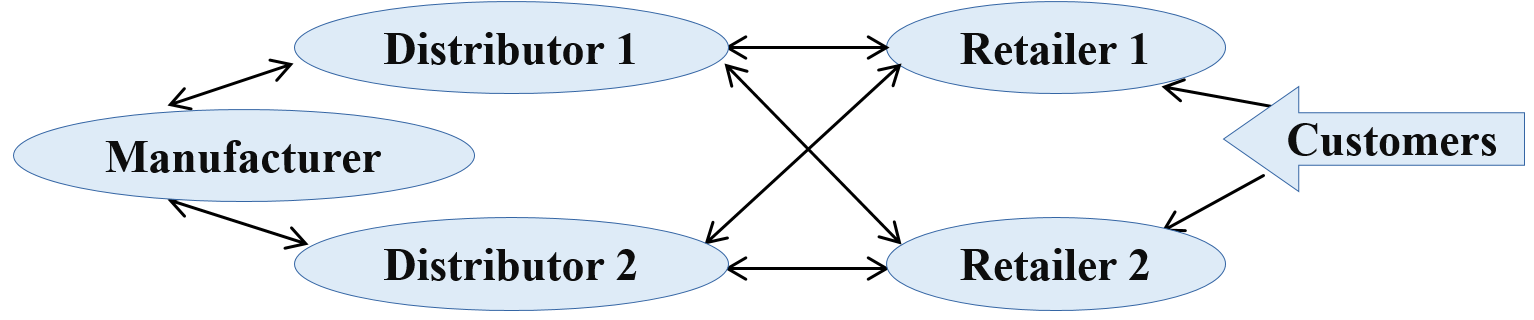
\epsfig{file = image/simple_supply_chain_net.png, width = 7.5cm}}
  \caption{A supply chain network with two retailers, two distributors and a manufacturer}
  \label{fig:simple_supply_chain_net}
  \vspace{-0.1cm}
\end{figure}

The demand arrival is modeled as a parameterized Python class with the attributes for selecting various distributions for arrivals and their parameters. For this case study, we assume that the arrivals are Poisson distributed, every customer purchases between 1 to 10 units, and the customer will choose retailer 1 with probability $p$, and retailer 2 with probability $(1-p)$. The retailers and distributors maintain an inventory with a typical $(s, S)$ policy. $s$ is the threshold below which the inventory will be restocked, and $S$ is the restocking level. Further, we add a behavior where a retailer will choose one of the distributors whose delivery cost is the least. The retailer will choose another distributor if the desired units are unavailable. If the necessary number of product units is unavailable, the retailer will refrain from placing an order for that particular day. A retailer makes a profit of $P$ units behind every unit sold. Whenever an inventory is restocked, it incurs a cost of $C$ units and a delay of $D$ days for the bulk order. Both these parameters differ for each pair of nodes in SC. Furthermore, an inventory holding cost is involved: $H$ units per day per item. If the holding cost $H$ is significant, it is reasonable to consider minimizing the inventory's capacity S. Figure \ref{fig:nomenclature} summarizes the model parameters and terminologies.

%\paragraph{Customer behavior:}
%The arrival of customers to retailers follows a Poisson distribution with an average arrival rate of $\lambda$. A customer purchases between 1 to 10 units from the retailer. If requested units are unavailable, the customer will cancel their purchase and return. A customer will choose any one of the available retailers with some probability $p$ to buy the product. It should be noted that the customers do not purchase the product directly from the distributors.
%\paragraph{Retailer behavior:}
%A retailer is directly connected to customers and facilitates product sales in the supply chain. Every retailer maintains an inventory to store product units, and the inventory behavior (discussed below) is followed. A retailer will choose any connected distributors whose delivery cost is the least to replenish its inventory. If desired units are unavailable at this distributor, the retailer will order from a distributor whose delivery cost is the next least one. If the necessary number of product units is unavailable, the retailer will refrain from placing an order for that particular day. A retailer makes a profit of $P$ units behind every unit sold.
%\paragraph{Distributor behavior:}
%A distributor holds massive units of products and facilitates the distribution to retailers all over a small town. A distributor has its inventory to stock up on the products and provide them to retailers whenever needed.  Every distributor maintains an inventory, which imitates the inventory behavior. 
%A distributor charges the retailer a delivery cost of $C$ whenever a delivery is made. The delivery is made in $D$ days, depending on the distance from the distributor to the retailer.
%\paragraph{Manufacturer behavior:}
%A manufacturer makes the product. There is only one manufacturer in the supply chain network. It is assumed that the manufacturer has abundant raw materials to produce the desired product. Additionally, it is assumed that the manufacturer can consistently produce and deliver the desired quantity of units to the distributors. A manufacturer charges the distributor a delivery cost of $C$ whenever a delivery is made. The delivery is made in $D$ days, depending on the distance from the manufacturer to the distributor.
%\paragraph{Inventory behavior:}
%A distributor or retailer can have inventory. The inventory has two parameters $(S,s)$ where $S$ represents the capacity and $s$ represents the inventory threshold. It has a simple replenishment policy as follows:
%\begin{itemize}
%    \item Inventory level is monitored daily and recorded at the end of the day. If it is low $(< s)$, a bulk order is placed to refill the inventory to level $S$.
%    \item A subsequent order is not placed until the previous order is fulfilled
%\end{itemize}
%Furthermore, an inventory holding cost is involved: H units per day per item. If the holding cost H is significant, then it is reasonable to consider minimizing the inventory's capacity S.

\begin{figure}[!h]
  \vspace{-0.2cm}
  \centering
   %\includegraphics[scale=0.40]{image/supply_chain_nemon.png}
   {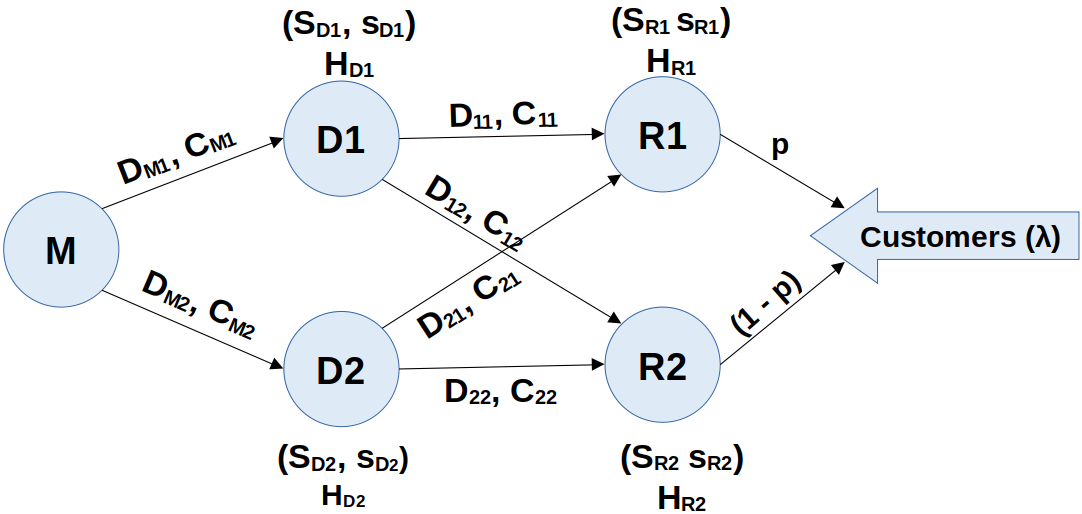
\epsfig{file = image/supply_chain_nomen.png, width = 7.7cm}}
  \caption{The figure depicts the model parameters and terminology used for the SC}
  \label{fig:nomenclature}
  \vspace{-0.1cm}
\end{figure}

%\paragraph{Nomenclature}
%Please refer to Figure \ref{fig:nomenclature} presented herein, where we provide a detailed discussion on the terminologies and nomenclature adopted to represent various components of the supply chain network.
%\begin{itemize}
%    \item The retailers and distributors in the supply chain are named from top to bottom, using a subscript index $i$. The network has two only retailers, $R_1$, $R_2$, and two distributors, $D_1$ and $D_2$. 
%    \item The probability of customers buying from retailer $R_1$ is denoted by $p$, so the probability that the customer will buy from $R_2$ is $(1-p)$.
%    \item For the inventory parameters $(S,s)$, subscript $R$ or $D$ represents whether the inventory belongs to a retailer or a distributor. It is followed by an index to pinpoint the retailer/distributor. The same naming policy is followed for the holding cost $H$ of the inventory. Therefore $(S_{R1}, s_{R1})$ are inventory parameters of the retailer $R_1$, and $H_{R1}$ is the associated holding cost.
%    \item $C_{ij}$ represents the delivery cost incurred from distributor $D_i$ to retailer $R_j$. Furthermore, $D_{ij}$ represents the delay in delivery. Therefore $C_{11}$ is a cost, and $D_{11}$ is the delay for delivery from distributor $D_1$ to retailer $R_1$.
%    \item  $M$ in the subscript is used if the delivery cost/delay is from the manufacturer to a distributor. ($C_{M1}$, $D_{M1}$ represents the delivery cost and delay from the manufacturer to $D_1$.
%\end{itemize}

%\paragraph{Parameter values}
%To ensure the reliability of the model, we have conducted validation tests for various parameter values. The maximum $surplus$ generated by the supply chain changes concerning the parameter values. Therefore values for arrival rate, delivery cost, inventory holding costs, and delivery delay are kept constant. It is assumed that the probability of a customer selecting any available retailer is constant and denoted by $p$. The following segment outlines the fixed parameter values used in our study:
%\begin{itemize}
%    \item The arrival rate of the customers ($\lambda$) is fixed at 20 customers per day.
%    \item The probability of a customer buying from retailer $R_1$ is  $p = 0.5 $ (So the probability of a customer buying from $R_2$ is $(1-p)=0.5$).
%    \item The inventory holding costs for retailers are $H_{R1} = H_{R2} = 10$ units, and for distributors, are $H_{D1} = H_{D2} = 1$ units.
%    \item The delivery costs from a distributor to a retailer are listed  as $C_{11} = 5000$, $C_{12} = 6000$, $C_{21} = 7000$, and $C_{22} = 5500$ units.
%    \item The delivery delays to deliver from distributor $i$ to retailer $j$ are $D_{11} = 2$ days, $D_{12} = 3$ days, $D_{21} = 3$ days, and $D_{22}=2$ days, respectively.
%    \item Finally, the delivery costs from manufacturer to distributors are $C_{M1} = C_{M2} = 500$, and delays are $D_{M1} = 7$ days, and $D_{M2} = 8$ days, respectively. 
%    \item $P = 100$ units is the profit generated per item the retailer sells.
%\end{itemize}
     
Out of these model parameters, we choose 8 as design parameters. These design variables and their bounds are summarized in \tablename ~ \ref{tab:param_val}. Other parameters are fixed at reasonable values.

\begin{table}[]\fontsize{9pt}{10pt}\selectfont
%\begin{table}[]
\caption{The Supply chain design parameters, their bounds and values}\label{tab:param_val}
\centering

%\begin{tabular}{|c|c|c|llll|}
%\hline
%\begin{tabular}[c]{@{}c@{}}Design\\ Parameters\end{tabular} & \begin{tabular}[c]{@{}c@{}}Lower\\ Bound\end{tabular} & \begin{tabular}[c]{@{}c@{}}Upper\\ Bound\end{tabular} & \multicolumn{4}{c|}{Values}                                                          \\ \hline
%$S_{R1}$                                                    & 350                                                   & 500                                                   & \multicolumn{1}{l|}{350} & \multicolumn{1}{l|}{400} & \multicolumn{1}{l|}{450} & 500 \\
%$s_{R1}$                                                    & 100                                                   & 250                                                   & \multicolumn{1}{l|}{100} & \multicolumn{1}{l|}{150} & \multicolumn{1}{l|}{200} & 250 \\
%$S_{R2}$                                                    & 350                                                   & 500                                                   & \multicolumn{1}{l|}{350} & \multicolumn{1}{l|}{400} & \multicolumn{1}{l|}{450} & 500 \\
%$s_{R2}$                                                    & 100                                                   & 250                                                   & \multicolumn{1}{l|}{100} & \multicolumn{1}{l|}{150} & \multicolumn{1}{l|}{200} & 250 \\
%$S_{D1}$                                                    & 600                                                   & 750                                                   & \multicolumn{1}{l|}{600} & \multicolumn{1}{l|}{650} & \multicolumn{1}{l|}{700} & 750 \\
%$s_{D1}$                                                    & 350                                                   & 500                                                   & \multicolumn{1}{l|}{350} & \multicolumn{1}{l|}{400} & \multicolumn{1}{l|}{450} & 500 \\
%$S_{D2}$                                                    & 600                                                   & 750                                                   & \multicolumn{1}{l|}{600} & \multicolumn{1}{l|}{650} & \multicolumn{1}{l|}{700} & 750 \\
%$s_{D2}$                                                    & 350                                                   & 500                                                   & \multicolumn{1}{l|}{350} & \multicolumn{1}{l|}{400} & \multicolumn{1}{l|}{450} & 500 \\ \hline
%\end{tabular}


\begin{tabular}{|c|c|c|}
\hline
\begin{tabular}[c]{@{}c@{}}\textbf{Design}\\ \textbf{Parameters}\end{tabular} & \begin{tabular}[c]{@{}c@{}}\textbf{Lower}\\ \textbf{Bound}\end{tabular} & \begin{tabular}[c]{@{}c@{}}\textbf{Upper}\\ \textbf{Bound}\end{tabular} \\ \hline
$S_{R1}$                                                    & 350                                                   & 500                                                   \\ \hline
$s_{R1}$                                                    & 100                                                   & 250                                                   \\ \hline
$S_{R2}$                                                    & 350                                                   & 500                                                   \\ \hline
$s_{R2}$                                                    & 100                                                   & 250                                                   \\ \hline
$S_{D1}$                                                    & 600                                                   & 750                                                   \\ \hline
$s_{D1}$                                                    & 350                                                   & 500                                                   \\ \hline
$S_{D2}$                                                    & 600                                                   & 750                                                   \\ \hline
$s_{D2}$                                                    & 350                                                   & 500                                                   \\ \hline
\end{tabular}

\end{table}
%The parameter values for inventory thresholds and capacities are adjustable and not predetermined. Assuming variable values for the inventory thresholds and capacities is reasonable as the retailer or distributor controls them to ensure the product's availability. \tablename~ \ref{tab:param_val} summarises the ranges of values for supply chain parameters $(S,s)$.
%The range of values these parameters can take are as follows: \\ 
%$S_{R1} \in [350,500]$, $s_{R1} \in [100,250]$, $S_{R2} \in [350,500]$, $s_{R2} \in [100,250]$, $S_{D1} \in [600,750]$, $s_{D1} \in [350,500]$, $S_{D2} \in [600,750]$, and $s_{D2} \in [350,500]$.

\paragraph{Model Implementation:}
We have implemented the model in a modular manner using SimPy library \cite{SimPy}. The SC nodes, such as retailers and distributors, are implemented as parameterized classes that are simply instantiated, the parameter values are fixed, and nodes are connected to model the supply chain's structure. The optimization study aims to maximize the net profit (surplus) generated by the supply chain, which is calculated as follows. In addition, each simulation run reports the performance measures as summarized in \tablename~\ref{tab:performance_measures}.

%We have modeled the system using the SimPy library \cite{SimPy}. The SC's manufacturer, distributor, customer or retailer is called a supply chain node. They exhibit similar behavior, placing orders with connected nodes when their inventory levels are low or serving connected nodes. We have implemented a class \textit{SC\_node} to model such behavior. The \textit{Container} class of SimPy is used to model inventory behavior. We override this class to monitor the inventory levels daily by implementing \textit{MonitoredContainer} class. In a single simulation run, we calculate various supply chain network performance measures, which are listed in \tablename~ \ref{tab:performance_measures}. They are calculated for each node in the supply chain, and the total profit generated is the aggregate of $P_{avg}$ generated by each node. Similarly, the supply chain cost is the aggregate of cost $C_{avg}$ incurred at each node. The supply chain $surplus$ thus is calculated as follows:

$$P'_{net} =Surplus=\sum_n{(P_{avg} - C_{avg})} = \sum_n{P_{net}}$$

Where $n$ represents a node in the system.
\begin{table}[]\fontsize{9pt}{10pt}\selectfont
%\begin{table}[ht]
\caption{Performance measures reported from every single simulation run}\label{tab:performance_measures} \centering
\begin{tabular}{|r|l|}
\hline
\multicolumn{1}{|c|}{\begin{tabular}[c]{@{}c@{}}\textbf{Performance}\\ \textbf{measures}\end{tabular}} & \multicolumn{1}{c|}{\textbf{Description}}                                                               \\ \hline
$F_{ret}$                                                                                  & \begin{tabular}[c]{@{}l@{}}Fraction of customers\\ returned due to unavailability\end{tabular} \\ \hline
$P_{avg}$                                                                                 & \begin{tabular}[c]{@{}l@{}}Average profit\\ generated per day\end{tabular}                     \\ \hline
$C_{H_{avg}}$                                                                                 & \begin{tabular}[c]{@{}l@{}}Average inventory\\ hold cost per day\end{tabular}                  \\ \hline
$C_{D_{avg}}$                                                                                 & \begin{tabular}[c]{@{}l@{}}Average delivery cost\\ per day\end{tabular}              \\ \hline
$C_{avg}$                                                                                 & \begin{tabular}[c]{@{}l@{}}Average cost incurred per\\ day $(C_{avg} = C_{H_{avg}} + C_{D_{avg}})$\end{tabular}   \\ \hline
$T_{avg}$                                                                                 & \begin{tabular}[c]{@{}l@{}}Average number of units\\ sold per day (Throughput)\end{tabular}    \\ \hline
$I_{avg}$                                                                                  & \begin{tabular}[c]{@{}l@{}}Timed-averaged number\\ of units in inventory\end{tabular}          \\ \hline
$P_{net}$                                                                                  & \begin{tabular}[c]{@{}l@{}}Average net profit per day\\ $(P_{net} = P_{avg} - C_{avg})$\end{tabular}     \\ \hline
\end{tabular}

\end{table}
Since the goal is to improve the average profit, it is necessary that the inventory parameters $(s, S)$ at all nodes are appropriately set. Having overly large inventory levels will incur a very large holding cost increasing the cost of the supply chain, whilst keeping very low inventory levels will result in a reduction in total profit generated in the supply chain. Thus it is essential to find the optimum parameter values under these assumptions. 
%We conducted simulations with varying simulation lengths and design configurations to validate the model's accuracy and evaluated the simulation log. Multiple modifications were made to the model and validated to replicate the exact behavior of the supply chain network we discussed above.
After developing a simulation model for the system, executing it for various input parameter values to perform optimization requires a significant computational effort. The number of simulations required to explore the entire design space depends on the number of input parameters and the range of values considered.
\paragraph{Computational Cost versus Accuracy trade-off:}
We estimate the impact of the length of each simulation run and the number of independent samples on the accuracy of the estimated performance measure. For a single point in the design space, we perform multiple simulation runs varying the length of each simulation run ($L$). For each value of $L$ we perform multiple ($N$) simulation runs with distinct randomization seeds to measure and obtain an estimate of the expected performance measure. This is necessary since the model is stochastic. We also measure the relative standard error (RSE) in the performance measure for each value of $L$ using $N$ samples. It is expected that the RSE is inversely proportional to $\sqrt(N)$ as the sample average is Normally distributed. Further, the RSE should reduce with $L$ if the performance metric is a long-run average measure for a model that has a steady-state behavior. Figure \ref{fig:compute_effort} presents the RSE values measured with respect to $L$ and $N$. Further, the computational cost is directly proportional to $L\times N$. The existence of such a plot enables the modeler to estimate the computational cost and budget the time available for design exploration for achieving a reasonable level of accuracy in simulation-based performance estimates.
%The model is stochastic since the arrival rate parameter of the system is a random variable. It is necessary to conduct multiple simulation runs to estimate the system's expected performance. Given the computational cost of the simulation, we need to determine the number of simulation runs that would yield an estimated expected value of the performance measure with an acceptably low error level. We utilize the Relative Standard Error (RSE) and Standard Error (SE) metrics to determine the number of simulations $(N)$ to be performed and the length $(L)$ required for estimating the expected value of the performance measure with an acceptable level of error. \tablename~ \ref{tab:computaional_effort} summarises the execution time required to run the simulation model for a specified duration of L days and N=60 simulation runs, for a random input parameter value $X =[S_{R1}, s_{R1}, S_{R2},s_{R2}, S_{D1},s_{D1}, S_{D2},s_{D2}]=[300,200,350,200,700,350,650,400]$. 
%We also computed the computational effort for $N=80$ and $N=100$ and generated a plot that depicts the trade-off between the computational effort and the accuracy of the estimated expected performance measure value. Please refer to Figure \ref{fig:compute_effort} for details. To evaluate the expected performance measures at a single point in the design space, we set the length parameter $L$ to 720, and the number of simulations $N$ to 60, resulting in a reasonable RSE of 0.34\% and a computational effort of around 130 seconds.
\begin{figure}[!h]
  \vspace{-0.2cm}
  \centering
   %\includegraphics[scale=0.40]{image/supply_chain_nemon.png}
   {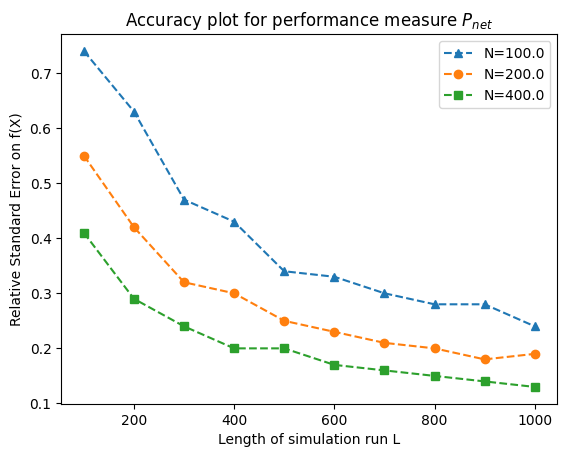
\epsfig{file = image/rse_vs_sim_len.png, width = 7.5cm}}
  %\caption{This figure illustrates the trade-off between the computational effort and the accuracy of the expected performance measure $P_{net}$.}
  \caption{Relative Std Error (RSE) in simulation-based performance estimate as a function of simulation run length $L$ and the number of samples $N$}
  \label{fig:compute_effort}  
\end{figure}
 For the optimization case study, we fix the simulation run length $L$ to 720 days and the number of simulation samples $N$ to 60, for reasonable accuracy (RSE = 0.34\%). This corresponds to a computational time of 130 seconds on a single-core x86 based modern workstation. Thus, evaluating the objective performance estimate $f(X)$ at any given point $X$ in the design space takes us approximately \textbf{130 seconds}.
\paragraph{Simulation-based measurements:} The purpose of the case study is to arrive at a rule of thumb on how many points are enough for the optimization process. We first measure at very densely spaced points, and then in later steps, we will incrementally see the impact of selecting a subset of these points for building the meta-model. So we sample the design space at regular space grids, considering four equispaced points along each dimension. This results in a total of $4^8 = 65536$ design points and gives us a simulation budget of approximately 96 days. To perform this in a reasonable amount of time, we perform simulations in parallel on an 80-core rack server using Python's Multiprocessing \cite{Multiprocessing} library. With a speed-up of $64$x, the data was obtained in approximately 2 days. This data is actual simulation data and no meta-model has been built on top of it. This raw data itself gives valuable information about the shape of the objective function.
%The execution time to evaluate the performance measures of the system at each point in the design space can be calculated as follows:
%$n^{k}*(t)$ = $150^8*130$ sec = $(2.5628*10^{17})$ sec. 
%$n$ is the total number of values a parameter can take, $k$ is the total number of parameters, and $t$ is the execution time to evaluate the system's expected performance measures at a single point in the design space. $150^8$ is enormous, and the design space is vast. Computing the system performance measures at every point in the design space is not feasible. We have assessed the system performance at discrete points in the design space, where each parameter $S$ and $s$ are restricted to four equidistant values within a specified range. For instance, the parameter $S_{R1}$ is limited to 350, 400, 450, and 500 values. We have considered all possible input parameter combinations resulting from this discretization (resulting in $4^8 = 65536$ design points). The execution time to evaluate performance measures at these points in the design space is $4^8*130=8519680~sec \approx 96.60$ days. We employed Python's Multiprocessing \cite{Multiprocessing} package to run the script concurrently on an 80-core rack server to expedite the computation time. As a result, we achieved a speedup of $64x$, and the data was obtained within approximately two days. The collected data was visualized to investigate the potential relationships between the input parameters and the resulting output performance measures.
\begin{figure}[!h]
    \begin{frame}{
    %\vspace{-0.2cm}
    \centering {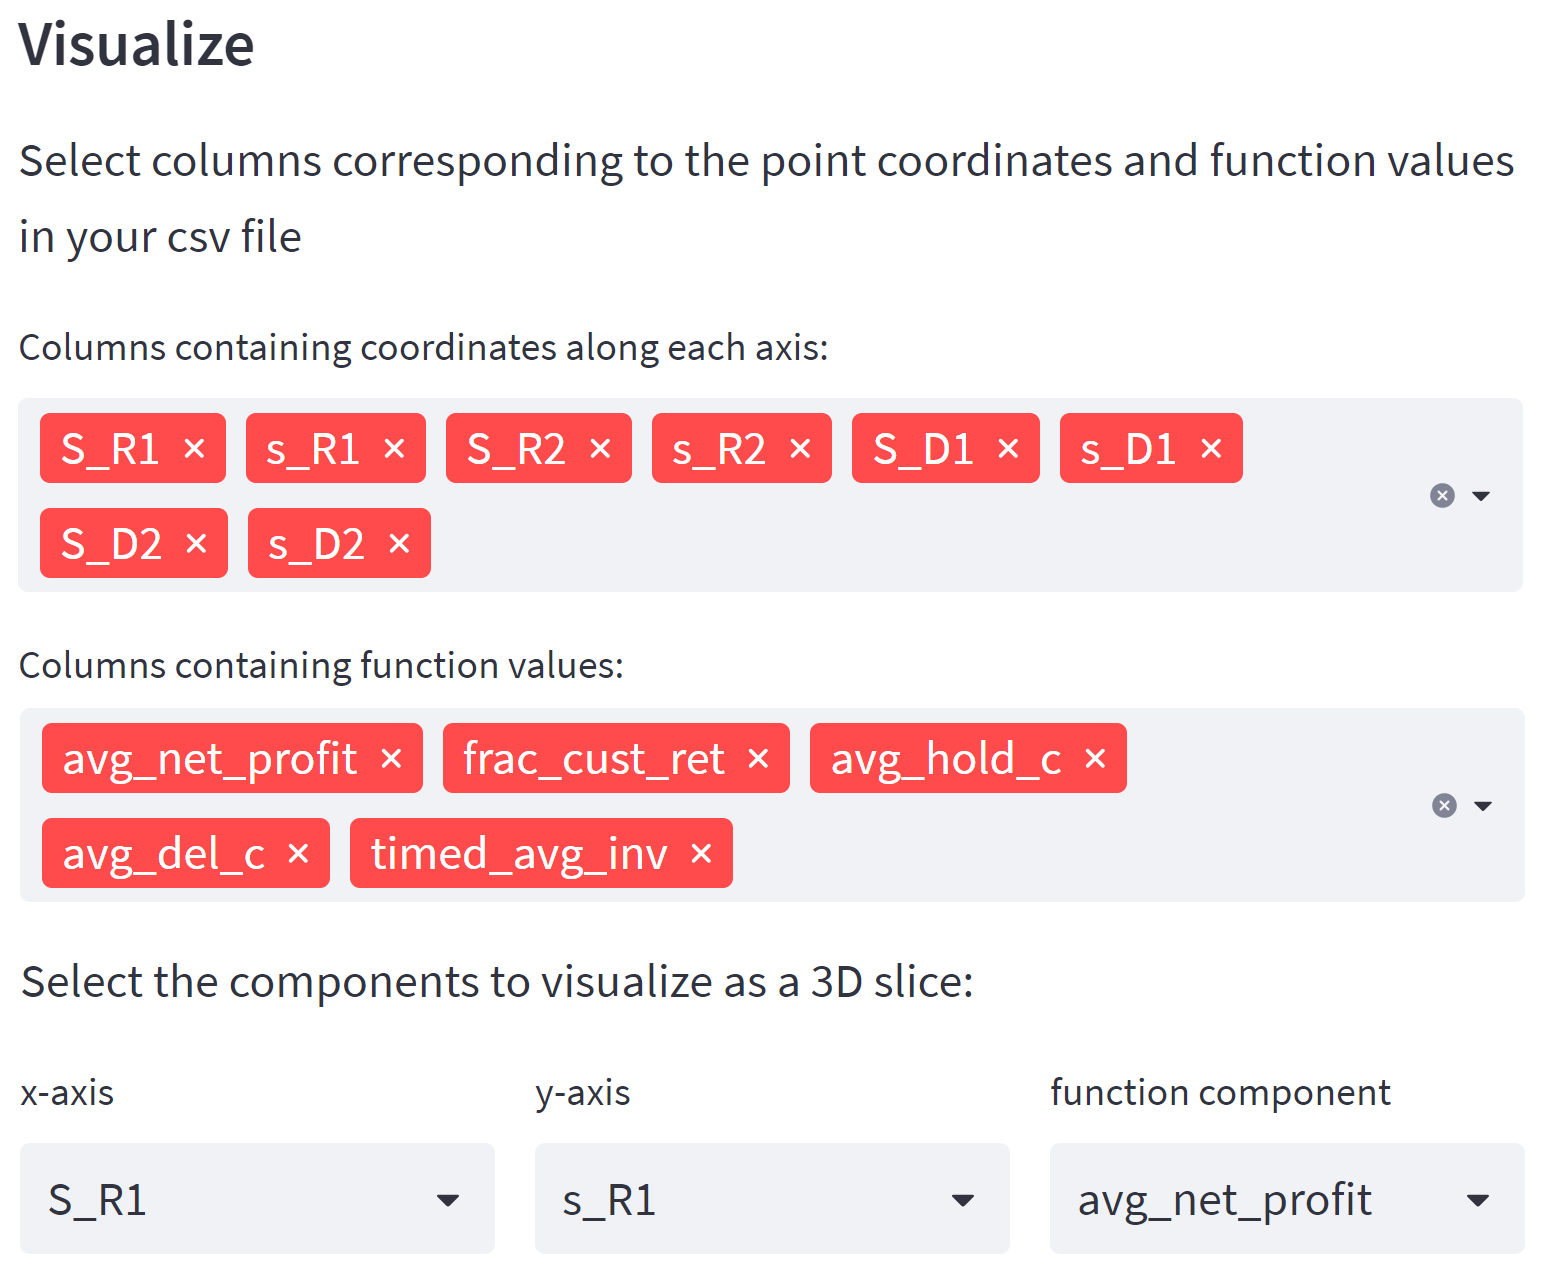
\epsfig{file = image/DataVis_params.png, width = 7.5cm}}  
    }
    \end{frame}
  \caption{Snapshot of \textit{DataVis} tool illustrate choosing input parameters and function values to visualize a 3D slice}
  \label{fig:DataVis_param_select}
  %\vspace{-0.1cm}
\end{figure}
\begin{figure*}[!t]  
  \hspace*{1.5cm}
  \begin{frame}{
    %\vspace{-0.2cm}
    \centering {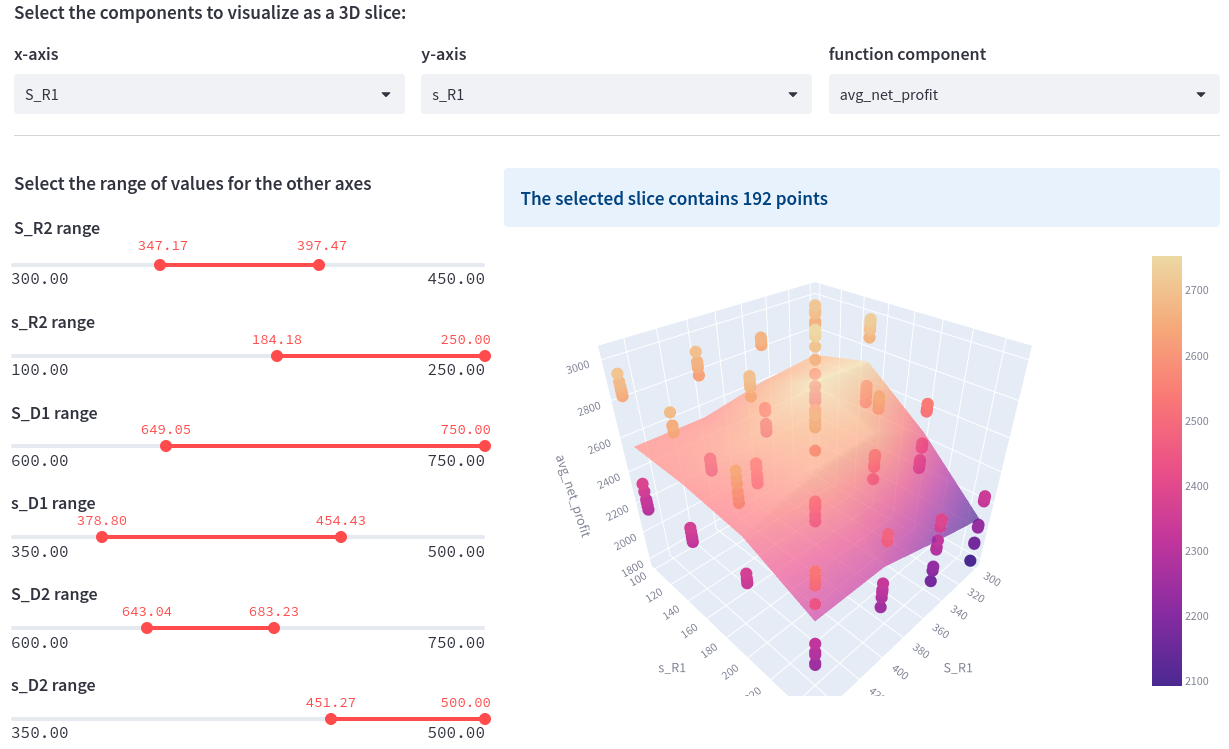
\epsfig{file = image/DataVis_slice.png, width = 13cm}}
    }
  \end{frame}
  \caption{The \textit{DataVis} tool snapshot displays a 3D slice with input parameter values $S_{R1}$, $s_{R1}$, and corresponding performance measure $P_{net}$ with interactive sliders for remaining parameters}
  \label{fig:DataVis_slice}
  %\vspace{-0.1cm}
\end{figure*}
\paragraph{Visualizing the design space:} 
Once the design space is sampled using a simulation model at regularly spaced grids, this data already provides insights into how the objective function varies with respect to varying input parameter values. However, this data is multidimensional, and $f(X)$ has multiple performance components summarized in Table \ref{tab:performance_measures}. Moreover, the input design space is multidimensional, 8 dimensions in this case, hence it becomes difficult to visualize. Several approaches exist to visualize multidimensional data, for example, Principle Component Analysis (PCA), clustering, etc. One approach is to visualize the data as a 3D slice by choosing two axes at a time and fixing values for other axes. The other axes' values can be varied on a slider to interactively see how the objective function surface moves with respect to different parameter values. A GUI tool makes this very simple and intuitive. We have implemented this functionality separately as a visualization tool called \textit{DataVis}. It is implemented using the Python Streamlit library. The visualizer tool allows the user to visualize a three-dimensional slice of the selected objective function by choosing two axes at a time (Figure \ref{fig:DataVis_param_select}) and fixing the values of the other axes on a slider, which can be interactively moved. Figure \ref{fig:DataVis_slice} shows the screenshot of the tool. The tool is hosted on a public repository. The tool can be used to visualize both the design space and meta-models.
%The data is multidimensional, and many system performance measures are of interest. Visualization of such multidimensional data can aid in exploiting the relation between input parameters and output measures. There is a need for such tools that allows us to explore multidimensional data. We have designed GUI front end to visualize the data called \textit{DataVis} \cite{karanjkar_2023} using \textit{streamlit} framework. The app is deployed on \textit{streamlit} platform and is open to all. It facilitates the visualization of slices of higher dimensional data in 3D. A user can upload a CSV file and choose input parameters and function values as shown in Figure \ref{fig:DataVis_param_select}. The obtained data is visualized with the help of \textit{DataVis}, Figure \ref{fig:DataVis_slice} shows a slice of data with input parameters $S_{R1}$, $s_{R1}$ and performance measure $P_{net}$ with other input parameter values fixed on the sliders. We observe low-order trends between the input parameters and the output performance measure, insights can be drawn on how $P_{net}$ varies with input parameters, and gradient information can be exploited to apply optimization methods.
\paragraph{Meta-model building and tuning:} The next step in the case study is to arrive at suitable design choices on how many measurements are necessary to build a meta-model with reasonable accuracy, what is the impact of the type of meta-model, and meta-model parameter value tuning. To perform this exploration, we consider NN and GPR meta-models. The number of hidden layers is fixed to 4 with 32 neurons for NN, and the length parameter is fixed to value 1 with bounds $(30,60)$ for RBF kernel of GPR meta-model by tuning process. Out of $2^8$ points, we select a larger and larger subset of the points as training points, with the remaining points as test points for building the meta-models. For each choice of the number of points we report the extent of the match with the test points as a mean squared error (MSE), this is summarized in Table \ref{tab:obtained_results}. We use the \textit{scikit-learn} \cite{scikit-learn} to build the meta-models. While they are currently tuned for the purpose of the case study, in the InventOpt tool, the user will be able to specify the meta-model parameters and tune them to obtain a reasonably good match with data.

To assess the impact of the choice of meta-models, we perform the optimization run described in the next section by building meta-models with successively larger subsets of the points. The insights are summarized in Section \ref{sec:results}.
%The generated data ($65536$ points) represents only a tiny fraction of the total design space. The maximum \textit{surplus} found among these data points is $f(X) = 3462.27$ at $X=[350,150,350,150,750,450,750,450]$. A meta-model is fitted to the data points obtained to model the relationship between the input parameters and output performance measures. The fitted meta-model is then used to optimize the system by applying gradient-based optimizers to find the best surplus in the entire design space. Gaussian Process Regression (GPR) and Neural Network (NN) models were fitted to the obtained data. The \textit{scikit-learn} \cite{scikit-learn} package in Python was utilized to construct the GPR and NN meta-models.
%A meta-model can be built using all the points in the design space. To reduce the computational complexity of evaluating the system's performance measures at each point in the design space, it is preferable to build a meta-model using the fewest possible number of points. We have experimented with randomly sampled 25\% ($16384$ points), 50\% ($32768$ points) and 75\% ($49152$ points) of the total points in the generated data. The time to evaluate the system's performance measures at these many points without parallel aid is approximately 24, 49 and 73 days, respectively. The computational expense is more if we decide to sample more points from the design space. However, with fewer points, the meta-model might be unable to capture the optimum in the design space. 
%Mean square error (MSE) is used to assess how well a meta-model $g(X)$ approximates the original $f(X)$ surface. The mean square error (MSE) is computed for all data points except the training points, wherein if a meta-model is constructed using 25\% of the data points, the remaining 75\% of points are utilized to determine the MSE. We conduct experiments with various meta-model parameter values and use \textit{DataVis} tool to visualize the fit. We select the parameter values that yield a meta-model that approximates the shape of the original surface with an acceptable MSE. The GPR meta-model is fitted with the RBF kernel function with parameter values \textit{length}=1 and \textit{length bounds} = (30,60). The NN meta-model has four hidden layers, each containing 32 neurons.
\begin{figure*}[!h]
     \centering
     \begin{subfigure}[b]{0.49\textwidth}
         \centering
         \caption{COBYLA}
         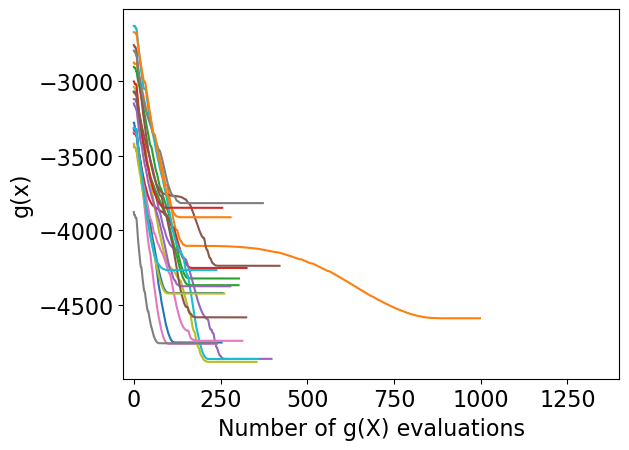
\includegraphics[width=\textwidth]{image/75gprCOBYLA_itrs.png}
         \label{fig:conv_cobyla}
     \end{subfigure}
     \hfill
     \begin{subfigure}[b]{0.49\textwidth}
         \centering
         \caption{Powell}
         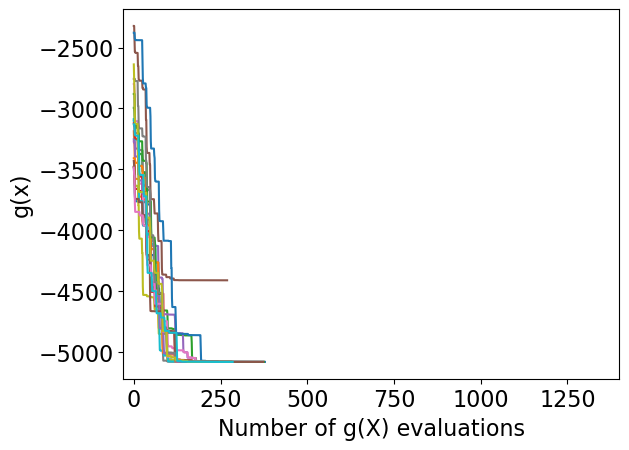
\includegraphics[width=\textwidth]{image/75gprPowell_itrs.png}
         \label{fig:conv_powell}
     \end{subfigure}
     \vfill
     \begin{subfigure}[b]{0.49\textwidth}
         \centering
         \caption{Nelder-Mead}
         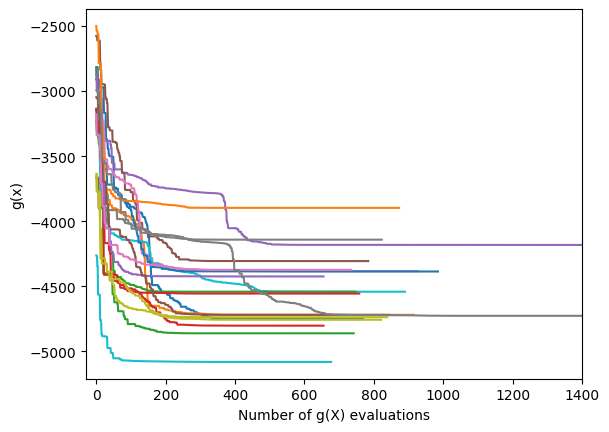
\includegraphics[width=\textwidth]{image/75gprNelderMead_itrs.png}
         \label{fig:conv_neldermead}
     \end{subfigure}
     \hfill
     \begin{subfigure}[b]{0.49\textwidth}
         \centering
         \caption{SLSQP}
         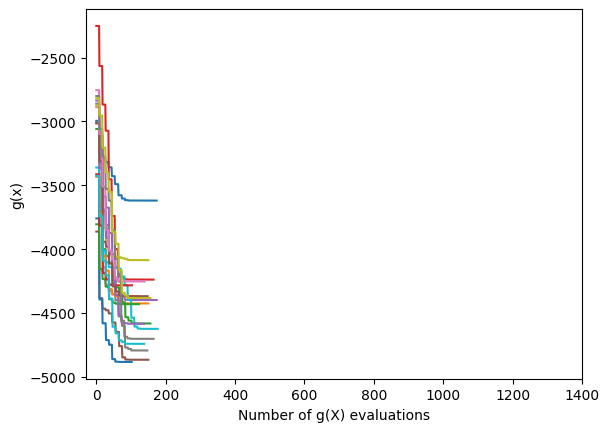
\includegraphics[width=\textwidth]{image/75gprSLSQP_itrs.png}
         \label{fig:conv_slsqp}
     \end{subfigure}
        %\caption{The convergence plots depict the performance of optimizers applied to the GPR meta-model with 75\% training data. Each coloured line signifies a run of the optimizer with a distinct random initial point $X_0$. Note that the objective is to maximize $g(X)$; thus, minimizing $-g(X)$ is attempted.}
        \caption{Convergence plots for various optimizers on the GPR meta-model with 75\% data.}
        \label{fig:convergence_plots}
\end{figure*}
\paragraph{Meta-model-based optimization:} The goal is to see which set of optimizers are well suited for optimization on top of a meta-model. For this, we consider all optimizers in SciPy.optimize \cite{2020SciPy-NMeth} library. Even if the design space is discrete valued the meta-model produces a continuous and smooth surface, therefore continuous optimizers can be applied, and they use gradient information. The optimizers used for the study are listed in Table \ref{tab:obtained_results}, out of these COBYLA and Powell are trust region-based methods, SLSQP and Nelder-Mead are gradient-based methods and are popular choices for black-box optimization problems. We choose to use local optimizers rather than global optimizers because the idea is to utilize gradient information to quickly converge to regions of interest. One can use global optimizers such as Simulated Annealing or Tabu search which are more suited when the objective function is erratic and lacks any trends. While this study only explores local optimizers, in the planned implementation, a few global optimizers will also be provided, such as Simulated Annealing. 
%The study employs four optimization algorithms provided by the open-source Python library \textit{SciPy}  \cite{2020SciPy-NMeth}: Constrained Optimization BY Linear Approximation (COBYLA), Sequential Least SQuares Programming optimizer (SLSQP), Nelder-Mead, and Powell. The following is a brief description of these optimizers.
%COBYLA is an iterative algorithm that uses linear approximations to the objective function and constraint functions to guide the search for the optimal solution. It is used for black-box optimization problems where the derivative of the objective function cannot be found. SLSQP is a gradient-based constraint optimization method. It is an iterative method, and the search direction and the step size are estimated at each iteration. Nelder-Mead is an unconstrained direct search optimization method and does not use derivative information to search for the optimum. Powell's optimization method can solve both constrained and unconstrained optimization problems. It is a derivative-based optimization method that combines line searches and trust regions to find the optimal solution. 
%\begin{landscape}
\begin{table*}[!t]\centering \setlength{\tabcolsep}{2pt} \fontsize{7pt}{9pt}\selectfont
\caption{The obtained results and reported optimum by applying different optimizers on GPR and NN meta-models}\label{tab:obtained_results}
% Please add the following required packages to your document preamble:
% \usepackage{multirow}
\begin{tabular}{|l|l|l|r|r|r|r|}
\hline
\multicolumn{1}{|c|}{\textbf{\begin{tabular}[c]{@{}c@{}}Training \\ Dataset\\ Size\end{tabular}}} & \multicolumn{1}{c|}{\textbf{MSE}} & \multicolumn{1}{c|}{\textbf{Optimizer}} & \multicolumn{1}{c|}{\textbf{\begin{tabular}[c]{@{}c@{}}Optimum\\ Objective\\ Value\end{tabular}}} & \multicolumn{1}{c|}{\textbf{\begin{tabular}[c]{@{}c@{}}Avg Number\\ of $g(X)$ \\ Evaluation\end{tabular}}} & \multicolumn{1}{c|}{\textbf{\begin{tabular}[c]{@{}c@{}}Avg Time to \\ Compute $g(X)$\\ (seconds)\end{tabular}}} & \multicolumn{1}{c|}{\textbf{\begin{tabular}[c]{@{}c@{}}Distance \\ to Reference\\ Solution $X’$\end{tabular}}} \\ \hline
\multirow{4}{*}{\begin{tabular}[c]{@{}l@{}}25\%\\ (16,385 training\\ points)\end{tabular}}        & \multirow{4}{*}{0.0008}           & COBYLA                                  & 4203.5                                                                                            & 355                                                                                                        & 0.0239                                                                                                          & 156.5                                                                                                          \\ \cline{3-7} 
                                                                                                  &                                   & Powell                                  & 4327.5                                                                                            & 346                                                                                                        & 0.0297                                                                                                          & 10.0                                                                                                           \\ \cline{3-7} 
                                                                                                  &                                   & SLSQP                                   & 4203.5                                                                                            & 172                                                                                                        & 0.0321                                                                                                          & 156.5                                                                                                          \\ \cline{3-7} 
                                                                                                  &                                   & Nelder-Mead                             & 4296.1                                                                                            & 861                                                                                                        & 0.0294                                                                                                          & 105.9                                                                                                          \\ \hline
\multirow{4}{*}{\begin{tabular}[c]{@{}l@{}}50\%\\ (32,768 training\\ points)\end{tabular}}        & \multirow{4}{*}{0.0015}           & COBYLA                                  & 4736.3                                                                                            & 318                                                                                                        & 0.0726                                                                                                          & 109.0                                                                                                          \\ \cline{3-7} 
                                                                                                  &                                   & Powell                                  & 4780.6                                                                                            & 348                                                                                                        & 0.0635                                                                                                          & 10.0                                                                                                           \\ \cline{3-7} 
                                                                                                  &                                   & SLSQP                                   & 4736.3                                                                                            & 149                                                                                                        & 0.0587                                                                                                          & 109.1                                                                                                          \\ \cline{3-7} 
                                                                                                  &                                   & Nelder-Mead                             & 4736.3                                                                                            & 878                                                                                                        & 0.0987                                                                                                          & 109.1                                                                                                          \\ \hline
\multirow{4}{*}{\begin{tabular}[c]{@{}l@{}}75\%\\ (49,152 training\\ points)\end{tabular}}        & \multirow{4}{*}{0.0037}           & COBYLA                                  & 4882.7                                                                                            & 339                                                                                                        & 0.0685                                                                                                          & 157.5                                                                                                          \\ \cline{3-7} 
                                                                                                  &                                   & Powell                                  & 5082.1                                                                                            & 314                                                                                                        & 0.0717                                                                                                          & 10.3                                                                                                           \\ \cline{3-7} 
                                                                                                  &                                   & SLSQP                                   & 4882.7                                                                                            & 145                                                                                                        & 0.0775                                                                                                          & 157.5                                                                                                          \\ \cline{3-7} 
                                                                                                  &                                   & Nelder-Mead                             & 5082.1                                                                                            & 869                                                                                                        & 0.0764                                                                                                          & 10.2                                                                                                           \\ \hline
\end{tabular}
\end{table*}
%\end{landscape}

Since we use local optimizers, to avoid getting stuck in a local optimum we perform multiple independent runs (20 in this case) with distinct initial points. Among all runs, we report the best optimum found. The convergence plots for the optimizer runs are illustrated in Figure \ref{fig:convergence_plots}. The computation cost of optimization is negligible since the optimizer invokes the meta-model $g(X)$ and not the original simulation model. We see that as the number of $g(X)$ evaluations made by the optimizer increases the best solution is found. The objective is to maximize $g(X)$ thus, minimizing $-g(X)$ is attempted. Figure \ref{fig:convergence_plots} shows that SLSQP and Powell are performing better in comparison, they converge faster than COBYLA and Nelder-Mead. However, COBYLA and Nelder-Mead have the advantage of being trust region-based methods and are resilient to noise. The optimal solution found by these optimizers is summarized in Table \ref{tab:obtained_results}. We identify the optimum reported by these results as a promising region and perform one more iteration. We narrowed the parameter ranges and restricted the search to a smaller region in the design space. Each parameter $S$ and $s$ are restricted to four equispaced values within these ranges. The maximum in this region is found at $X' = [S_{R1}=320, s_{R1}=130, S_{R2}=325, s_{R2}=125, S_{D1}=735, s_{D1}=480, S_{D2}=735, s_{D2}=475]$ with $f(X') = 3546.26$. The final column in Table \ref{tab:obtained_results} shows the Euclidean distance between found optimum and $X'$ as a goodness of fit measure of the meta-model. The results were again visualised using the \textit{DataVis} tool. The meta-model-based optimization process was repeated for this new data set. However, the obtained results showed no significant improvement in the optimum $X'$. The following section presents a comprehensive analysis of the results obtained from the case study and the insights derived from it.
%The ranges for the parameters $S$ and $s$  are adjusted to $S_{R1} \in [310,325], s_{R1} \in [115,130], S_{R2} \in [310,325], s_{R2} \in [115,130], S_{D1} \in [720,735], s_{D1} \in [470,485], S_{D2} \in [720,735], s_{D2} \in [470,485]$.  We execute the simulation model with the input parameter values restricted to this region to identify the maximum within this constrained design space. It is observed to be present at $X' = [320, 130, 325, 125, 735, 480, 735, 475]$ with $f(X') = 3546.26$. The results were again visualised using the \textit{DataVis} tool. The meta-model-based optimization process was repeated for this new data set. However, the obtained results did not show any significant improvement in the optimum $X'$ found. The following section presents a comprehensive analysis of the results obtained from the case study and the insights derived from it.
%The present study employs the Bayesian Optimization method to estimate the optimal input parameter values that maximize the \textit{surplus} of the supply chain. Gaussian Process Regression (GPR) and Neural Network (NN) meta-models are utilized to obtain the posterior distribution via the application of the Bayes rule. Subsequently, various optimizers instead of acquisition functions are employed to determine the next promising region. A sampling of a limited number of points within the promising region is performed, followed by the application of the process of meta-model-based optimization. This iterative approach is repeated until the optimal solution within the design space is achieved. The process is detailed below.
%The optimizers are applied to both the GPR and NN meta-models, utilizing randomly sampled training datasets of 25\%, 50\%, and 75\% of the generated data. The results are summarized in \tablename~\ref{tab:obtained_results}. The highlighted cell indicates the optimized value determined by the optimizer, which is observed to be outside the predefined boundaries. Such found optimum is discarded. A performance discrepancy is observed between the Nelder-Mead optimizer and the NN meta-model. The column `optimum $g(X)$' refers to the optimum $P_{net}$ found by the optimizer on the respective meta-model. The next column lists the execution time taken for an optimizer to converge. The last column $d(X,X')$ lists the Euclidean distance between optimum $X$ found by the respective optimizer and the original optimum $X'$ mentioned below.
%The outcomes indicate that the maximum surplus values reported substantially deviate from the previously identified value of 3462.27, representing the maximum value in data obtained by running the simulation model. In addition, the reported optimal input parameter values exhibit considerable differences. These observations prompt redirecting the search for the optimum towards a more narrowly defined region, where a few additional points are sampled. This constitutes one iteration of the Bayesian optimization process.